\documentclass[journal=jacsat,manuscript=article]{achemso}
% Image-related packages
\usepackage{graphicx}
\usepackage{subcaption}
\usepackage[export]{adjustbox}
\usepackage{wrapfig}
\usepackage[version=4]{mhchem}
\usepackage[numbers]{natbib} % Use natbib for citations

\newcommand*\mycommand[1]{\texttt{\emph{#1}}}

\author{Nayanika Das}
\affiliation[UVicUCC]{Computational Biochemistry and Biophysics Lab, Research Group on Bioinformatics and Bioimaging (BI$^2$), Department of Biosciences, Universitat de Vic - Universitat Central de Catalunya, 08500 Vic, Spain}
\author{Other Authors}
\affiliation{Here is where the other authors work}
\author{Jordi Villà-Freixa}
\email{jordi.villa@uvic.cat}
\affiliation[UVicUCC]{Computational Biochemistry and Biophysics Lab, Research Group on Bioinformatics and Bioimaging (BI$^2$), Department of Biosciences, Universitat de Vic - Universitat Central de Catalunya, 08500 Vic, Spain}
\alsoaffiliation{IRIS-CC}

\title[Evolutionary trends of GPX6 $\Delta G^{\ddagger}$]
  {Computational analysis of the evolution of glutathione peroxidase 6 (GPX6) activation free energy}

\abbreviations{IR,NMR,UV}
\keywords{Ancestral enzyme reconstruction, enzyme design, empirical valence bond, free energy calculations}

\begin{document}
\maketitle 

\begin{abstract}
This study explores the computational analysis of glutathione peroxidase 6 (GPX6) activation free energy, emphasizing the evolutionary trends of selenium incorporation in enzymatic reactions. We discuss the mechanistic insights gained from various computational methods, including empirical valence bond (EVB) modeling, and their implications for understanding enzyme evolution.
\end{abstract}

\section{Introduction}

Selenium (Se), in the form of selenocysteine (Sec, U—the 21st amino acid) occurs in 25 proteins in the human proteome. Insertion of Sec into a protein is much more complicated than the other 20 amino acids because a UGA stop codon must be recoded as a sense codon for Sec \cite{Hondal2011}. The complexity of this process signifies that Sec must fulfill a chemical function that exerts biological pressure on the genome to maintain the Sec-insertion machinery \cite{Hondal2011, Cardey2007}. The view of Sec as a sophisticated innovation implies that for each occurrence of Sec in an enzyme, there is a unique and specific reason for the use of Se to enhance the enzymatic reaction relative to that of S \cite{Hondal2011}. This view also implies that since Se “speeds reactions,” Sec should have widely substituted for Cys in enzymes, which clearly has not occurred. Specific reasons for the usage of Sec might include the enhanced nucleophilic character of Se relative to S, or another might be the much lower pKa of a selenol relative to that of a thiol \cite{Hondal2011}. Although the catalytic triad of glutathione peroxidase (GPX) has been well recognized, there has been little evidence for the relevance of the interactions among the triad amino acids, i.e., selenocysteine (U), glutamine (Q), and tryptophan (W). Hence, the mechanism has been studied in various aspects. GPXSec activity classically reduces hydroperoxides, particularly hydrogen and lipid peroxides, with glutathione (GSH) as a cofactor \cite{Rees2024}. GPXCys containing proteins act on alternative substrates for peroxidation and may have additional functions, including signaling and oxidative protein folding. Thus, all GPX proteins may protect cells from oxidative stress \cite{Rees2024}. 

\subsection{Mechanism of GPX}

A catalytic mechanism proposed for GPX3 by Morokuma et al. based on DFT calculations has the resting state of Sec as selenol. In the first part of this reaction, hydrogen peroxide coordinates to the active site of the enzyme and the proton transfer is happening to the Gln83 residue \cite{Prabhakar2006, Prabhakar2005}. Morokuma \cite{Prabhakar2006} did an ONIOM(QM:MM) method to evaluate the quantitative effect of the protein surroundings on the energetics of an enzymatic reaction. In the first step, the formation of the selenolate anion \({\ Se^-}\) occurs via the proton transfer from the Se through the oxygen (O1) atom of hydrogen peroxide to the neighboring Gln83, leading to the intermediate (III) \cite{Prabhakar2006}. The computed barrier for the creation of the selenolate anion is 16.4 kcal/mol \cite{Prabhakar2006}. In the second step of the stepwise mechanism, the O1-O2 bond of $\ce{H_2O_2}$ is cleaved. During this process, one hydroxyl fragment (O1H) is transferred to the selenolate anion \({\ Se^-}\) to form selenenic acid (R-SeO1H), while simultaneously the second hydroxyl fragment (O2H) accepts the previously transferred proton from Gln83 to form a water molecule (IV). The overall barrier (from II to IV) for the formation of selenenic acid (E-Se-OH) becomes 18.0 kcal/mol \cite{Prabhakar2006}.

\begin{figure}[h]
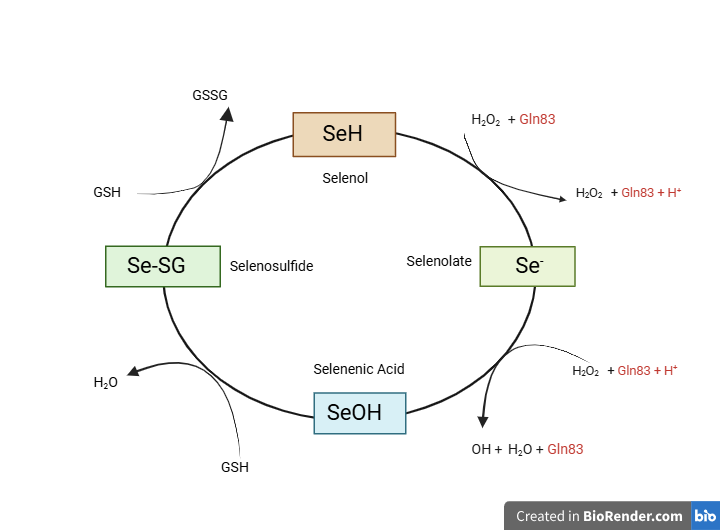
\includegraphics[width=0.7\textwidth]{/home/hp/nayanika/github/GPX6/figures/Catalytic_cycle.png}
\caption{Catalytic Cycle of GPX as given by Morokuma et al. where the resting state of selenium is selenol.}
\label{fig:figure1}
\end{figure}

\begin{wrapfigure}{h}{0.7\textwidth}
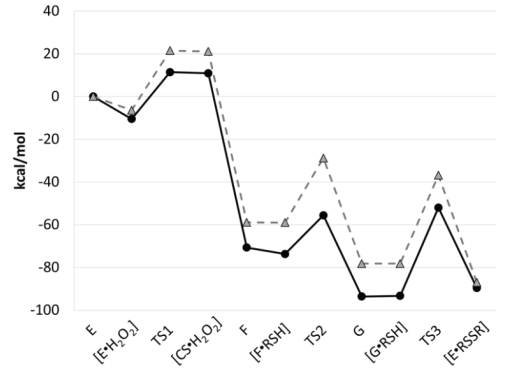
\includegraphics[width=0.7\linewidth]{/home/hp/nayanika/github/GPX6/figures/flohe_energyprofile.png} 
\caption{Energetic profile of the cycle for a SecGPX and the corresponding Cys, as DFT-calculated.}
\label{fig:figure2}
\end{wrapfigure}

\begin{figure}[h]
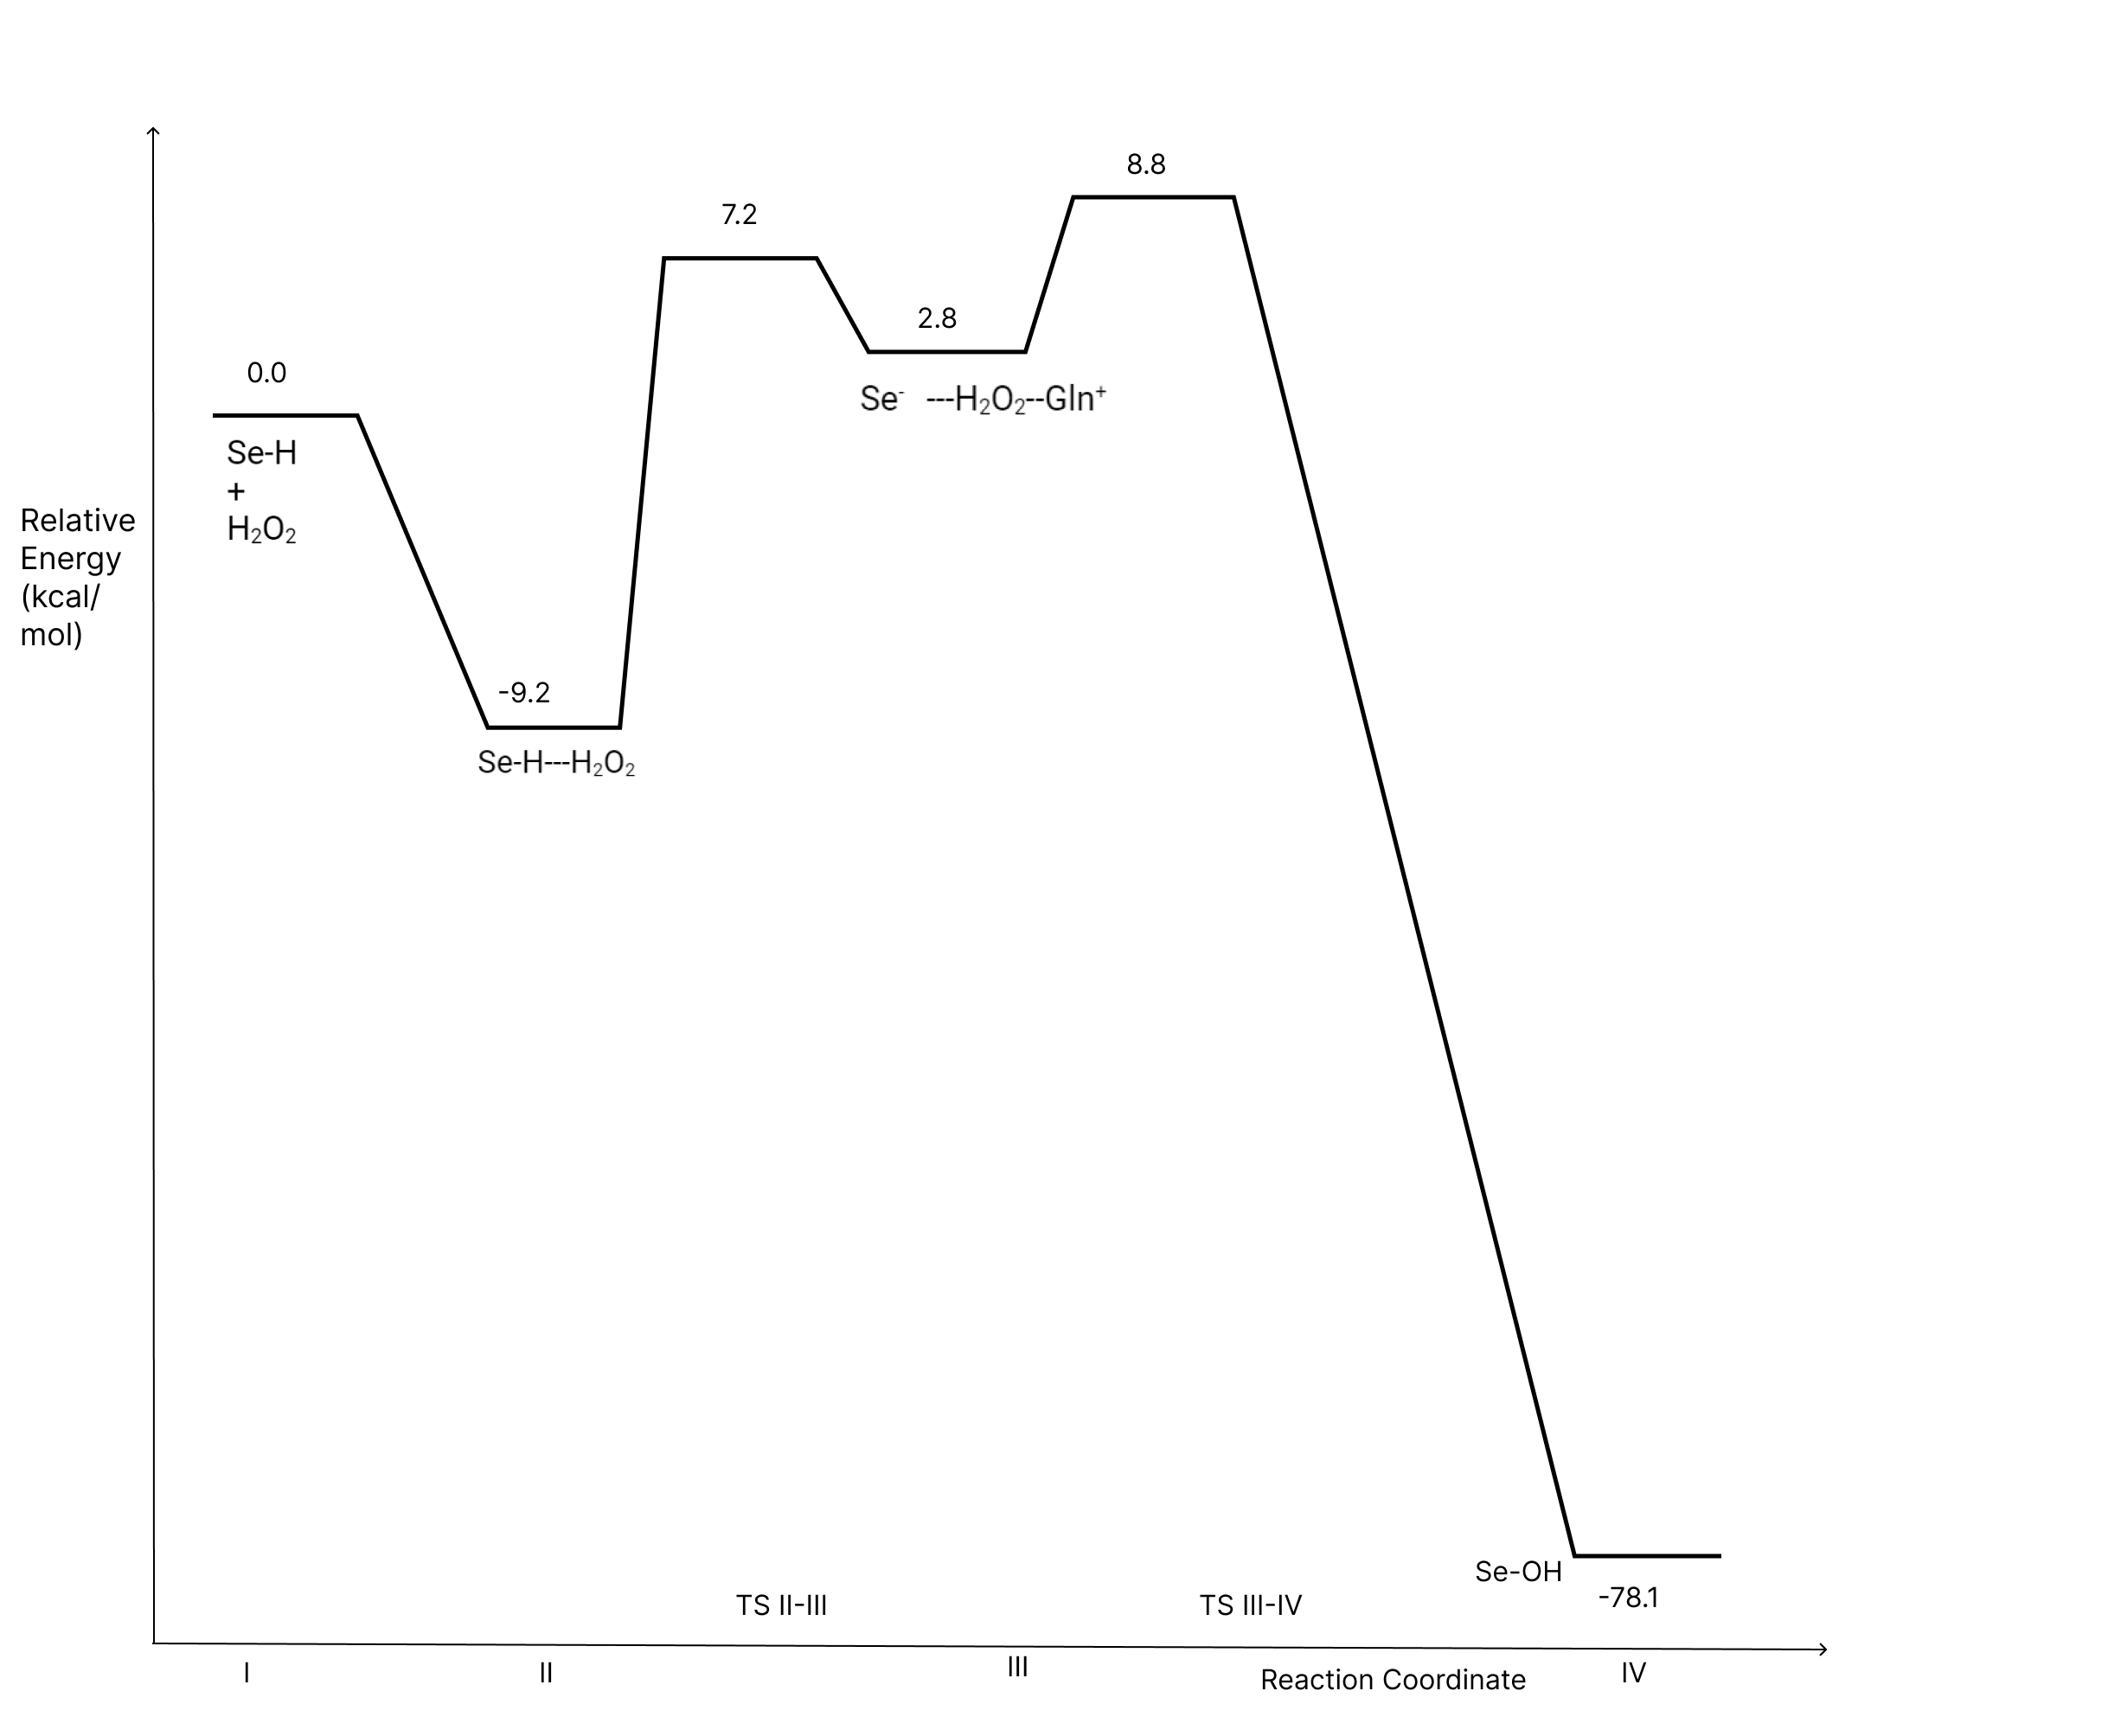
\includegraphics[width=0.7\textwidth]{/home/hp/nayanika/github/GPX6/figures/morokuma_energy_profile.png}
\caption{Potential Energy Diagram for the hydrogen peroxide reduction mechanism by GPX by Morokuma et al.}
\label{fig:figure3}
\end{figure}

Flohe et al. \cite{Orian2015} explored the mechanism in a different way wherein the selenocysteine proton moves via water to the indole nitrogen of the Trp residue and then the hydrogen peroxide, resulting in the formation of the products instantly. They show essentials of the DFT-calculated oxidation of SecGPX by $H_{2} O_{2}$. The calculation was performed with E, as shown in the figure, but with a single water molecule and $H_{2} O_{2}$ bound to the reaction center \cite{Orian2015}. The transition state, leading to the charge-separated form CS, involves three concurrent steps. CS evolves to the selenenic form F and a water molecule \cite{Orian2015}. The formation of the charge-separated form does not depend on the binding of $H_{2} O_{2}$ but just on the presence of water. Binding of $H_{2} O_{2}$ to CS then generates the identical unstable CS•$H_{2} O_{2}$ complex, which decays as described \cite{Orian2015}. In the transition state (TS1), the selenol proton moves via $H_{2} O_{2}$ and water to the Trp nitrogen, thus creating a charge-separated species. The resulting complex [CS•$H_{2} O_{2}$] is less stable than [CS], and can then decompose to create the product \cite{Orian2015}. 

\section{EVB Model}

One of the major challenges inherent to all QM/MM approaches is the high computational cost associated with the QM part of the calculation \cite{Carvalho2014}. This is important when it comes to QM/MM free energies where extensive conformational sampling is required. When one tries to deploy extensive DFT calculations to the QM region, this makes the cost of the computation much higher \cite{Carvalho2014}. So, we come to a hybrid QM/MM method using the empirical valence bond (EVB), which has proven to be very useful for calculating thermodynamic activation parameters for chemical reactions \cite{Oanca2024}. Certainly, EVB can capture the changes in the environment around the protein with a simple force field description and not a large DFT or QM/MM cluster, giving an idea of how the enzyme proceeds to work under certain environmental conditions \cite{Oanca2024}. If the activation free energy is correctly predicted at a given temperature, this just means that the sum of \(\Delta H\) and \(-T\Delta S\) is correctly predicted. A recent change that has been made is for cases where the reference reaction would be rather complex to parameterize the EVB potential energy surface directly on DFT calculations \cite{Oanca2024}. To understand the origin of the thermodynamic activation parameters in the EVB model, it is convenient to consider the simple form of the potential energy:

\begin{equation}
    E_{EVB} =  E_{0} + \sum_{i=1}^{N} \frac{1}{2} k_i \Delta x_i^{2} + V_{0}
\end{equation}
where \(\Delta x_i\) represents the deviation of the reaction coordinate (RC) from its equilibrium value, \(E_0\) is the energy of the equilibrium system, and \(V_0\) is an arbitrary constant energy \cite{Oanca2024}. 

In addition to capturing the free energy barrier for the reaction, it is also possible to derive the activation enthalpy and entropy from the simulations performed using EVB \cite{Oanca2024}. This would give better insight into how the mechanistic behavior changes from Cys to Sec in GPX. 

\section{Conclusion}

In summary, GPX can serve as an enzyme model for the evolution of Se to Cys, as there has been a lot of insight into the mechanistic behavior of GPX. Understanding how the protein interacts and recognizes the substrate can be crucial in predicting the enzymatic behavior. 

\section{References}
\bibliographystyle{unsrt} 
\bibliography{/home/hp/nayanika/github/GPX6/manuscript/references.bib}

\end{document}
